\chapter{$\chi$-omezenost}

\begin{notation}
	$\chi(G) = $ barevnost $G$ a $\omega(G) = $ klikovost $G$.
\end{notation}

\begin{observ}
	$\forall G: \chi(G) \geq \omega(G)$.
\end{observ}

\begin{defn}
	Grafová třída je $\chi$-omezená, pokud $\exists f : \N \to \N$ $\forall G$ graf z dané třídy platí $\chi(G) \leq f(\omega(G))$.
\end{defn}

\begin{example}
	$\chi$-omezené třídy: úplné grafy, rovinné grafy (funkce $f$ je konstantní), perfektní grafy.
\end{example}

\begin{observ}
	Intervalové, permutační, chordální, comparability, $\dots$ jsou perfektní a tudíž i $\chi$-omezené.
\end{observ}

\begin{observ}
	Circular-Arc grafy splňujé: $\chi(G) \leq 2 \omega(G)$.
\end{observ}

\begin{proof}
	Na kružnici máme intervaly. V jednom bodě kružnici rozstřihneme a obarvíme $\omega(G)$ barvami. Potom už máme jen intervalový graf, který je perfektní.
\end{proof}

\begin{defn}
	Následující definice jsou si ekvivalentní:
	
	\begin{itemize}
		\item $G \ in \text{CIR}$.
		\item $G$ je průnikový graf sečen v kružnici.
		\item $G$ je průnikový graf půlkružnic nad $x$-ovou osou.
		\item $G$ se dá reprezentovat posloupností čísel, kde se každé číslo $1, \dots, n$ vyskytuje právě dvakrát a platí, že vrcholy $v_i, v_j$ spolu sousedí právě když ta posloupnost obsahuje podposloupnost $i,j,i,j$ nebo $j,i,j,i$.
	\end{itemize}
\end{defn}

\begin{thm}
	$\text{CIR}$ je $\chi$-omezená.
\end{thm}

\begin{notation}
	Pro $k \in \N$ definujeme $\text{CIR}(k) := \{G \in \text{CIR}: \omega (G) \leq k\}$.
\end{notation}

\begin{observ}
	$\text{CIR}(k) \subseteq \text{CIR}(k+1) \subseteq \dots \subseteq \text{CIR}$.
\end{observ}

Chceme dokázat, že $(\forall k \in \N) \ (\exists f(k) \in \N) \ : \forall G \in \text{CIR}(k)$ platí, že $\chi(G) \leq f(k)$.

\begin{defn}
	Mějme $G \in \text{CIR}$ reprezentovaný jako průnikový graf půlkružnic. Pro $p,q \in \N_0$ $(p,q)$\textbf{-konfigurace} je množina $p+q$ vrcholů $x_1, \dots, x_p, y_1, \dots, y_q$ takové, že půlkružnice mají tuto vzájemnou polohu zobrazenou na obrázku \ref{konf}.
	
	\begin{figure}[!ht]\centering
		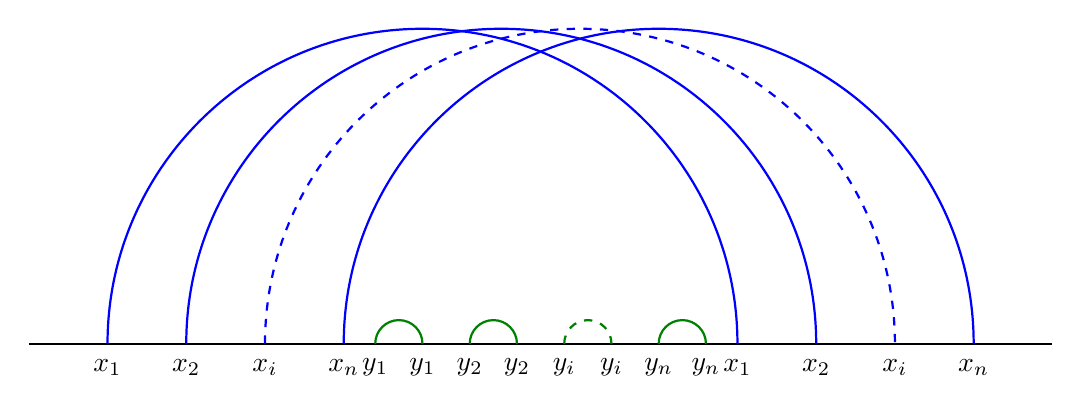
\begin{tikzpicture}
			\draw[thick] (0,0) -- (13,0);
			\draw[color=Blue, thick] (1,0) arc (180:0:4);
			\draw[color=Blue, thick] (2,0) arc (180:0:4);
			\draw[color=Blue, thick, dashed] (3,0) arc (180:0:4);
			\draw[color=Blue, thick] (4,0) arc (180:0:4);
			\draw[color=Green, thick] (4.4,0) arc (180:0:.3);
			\draw[color=Green, thick] (5.6,0) arc (180:0:.3);
			\draw[color=Green, thick, dashed] (6.8,0) arc (180:0:.3);
			\draw[color=Green, thick] (8,0) arc (180:0:.3);
			\node at (1, -.3) {$x_1$};
			\node at (2, -.3) {$x_2$};
			\node at (3, -.3) {$x_i$};
			\node at (4, -.3) {$x_n$};
			\node at (4.4, -.3) {$y_1$};
			\node at (5, -.3) {$y_1$};
			\node at (5.6, -.3) {$y_2$};
			\node at (6.2, -.3) {$y_2$};
			\node at (6.8, -.3) {$y_i$};
			\node at (7.4, -.3) {$y_i$};
			\node at (8, -.3) {$y_n$};
			\node at (8.6, -.3) {$y_n$};
			\node at (9, -.3) {$x_1$};
			\node at (10, -.3) {$x_2$};
			\node at (11, -.3) {$x_i$};
			\node at (12, -.3) {$x_n$};
		\end{tikzpicture}
		\caption{Definice $(p-q)$-konfigurace.}
		\label{konf}
	\end{figure}
\end{defn}

\begin{notation}
	$\text{CIR}(k,p,q) = \{G \in \text{CIR}, \omega(G) \leq k, G \text{ má reprezentaci bez } (p,q)\text{-konfigurace}\}$.
\end{notation}

\begin{observ}
	Pro $p > k$ a libovolné $q \in \N_0$: $\text{CIR}(k,p,q) = \text{CIR}(k)$.
\end{observ}

\begin{claim}
	$\forall k \in \N \ \forall p, q \in \N_0 \ \exists g(k,p,q) \in \N$ t.ž. $\forall G \in \text{CIR}(k,p,q) : \chi(G) \leq g(k,p,q)$.
\end{claim}

\begin{observ}
	Důkazem tohoto tvrzení platí věta.
\end{observ}

\begin{proof}
	Dané tvrzení dokážeme pomocí dvojité indukce: Indukcí podle $p \in \N_0$:
	
	\begin{lemma}
		$\forall G \in \text{CIR}(k,0,q) : \chi (G) \leq k (q-1)$ pro $q \geq 2$.
	\end{lemma}
	
	\begin{proof}[Proof of lemma]
		Indukcí podle $q \in \N_0$. Pokud $q = 2$ tak můžeme pozorovat, že všechny obloučky protínají společnou souvislou přímku. Tím pádem $\forall k : \text{CIR}(k,0,2) \subseteq \text{PER}$ které jsou perfektní.
		
		Nyní nechť $q > 2$. Nechť $G \in \text{CIR}(k, 0, q)$, vrcholy $G$ rozdělíme na 2 části $V_1, V_2$ tak, že
		
		\begin{itemize}
			\item $V_1$ bude indukovat graf z $\text{CIR}(k,0,2)$ a
			\item $V_2$ bude indukovat graf z $\text{CIR}(k,0,q-1)$.
		\end{itemize}
		
		Označme $\pi$ jakožto nejpravější konec obloučku. Potom $V_1$ jsou vrcholy, které mají levý konec vlevo od $\pi$. A $V_2$ jsou vrcholy, které mají levý konec napravo od $\pi$. Pak už použijeme indukci.
	\end{proof}
	
	\begin{lemma}
		Nechť $p \geq 1, q \geq 1$. Potom $\forall G \in \text{CIR}(k,p,q):$ vrcholy $G$ lze rozdělit na 2 části $V_A, V_B$ tak, že každá komponenta $G[V_A]$ i $G[V_B]$ patří do $\text{CIR}(k, p-1, 2q+1)$.
	\end{lemma}
	
	\begin{cor}
		Lze vzít $g(k,p,q) = g (k, p-1, 2q+1)$ tedy tvrzení pak platí.
	\end{cor}
	
	\begin{proof}[Proof of lemma]
		Mějme $G \in \text{CIR}(k,p,q)$. BÚNO: $G$ je souvislý a máme danou repre-\\zentaci. Nechť $x_0$ je vrchol $G$ jehož oblouček má nejlevější levý konec. Definujeme $V_i := \{x \in V(G) : \text{ nejkratší cesta v } G \text{ od } x_0 \text{ do } x \text{ má délku } i\}$.
		
		\begin{observ}
			Pokud vede hrana z $V_i$ do $V_j$ tak $|i - j| \leq 1$.
		\end{observ}
		
		\begin{observ}
			Z každého vrcholu $V_{i+1}$ vede aspoň 1 hrana do $V_i$.
		\end{observ}
		
		Nyní tvrdíme, že žádná komponenta $G[V_i]$ neobsahuje $(p-1, 2q + 1)$-konfiguraci.
		
		Nechť $C$ je komponenta $G[V_i]$ pro spor obsahující $(p-1, 2q + 1)$-konfiguraci. Označme $y_{q+1}$ nějaký oblouček $w$ musí protnout $y_{q+1}$, tedy $w \in V_{i-1}$. Aspoň jeden konec je mimo $C$. $V_{i-1} = V_0$ tedy hotovo. Kdyby měl oba konce v $C$, tak nelze protnout oblouček z $V_{i-2}$.
		
		Nyní nechť $x_1, \dots, x_{p-1}, y_{1}, \dots, y_{2q+1}$ je $(p-1, 2q + 1)$-konfigurace. Nechť $I$ je interval mezi nejlevějším a nejpravějším koncem obloučku v $C$.
		
		\begin{observ}
			Každý soused $w \in V_{i-1}$ vrcholu $y_{q+1}$ musí mít jeden konec mimo $I$.
		\end{observ}
		
		Potom $w, x_1, \dots, x_{p-1}, y_{1}, \dots, y_q$ nebo $w, x_1, \dots, x_{p-1}, y_{q+2}, \dots, y_{2q+1}$ je $(p,q)$-konfi-\\gurace v $G$, což je spor.
		
		Závěrem $V_{A} := \cup_{i \text{ sudé}} V_{i}$ a $V_{B} := \cup_{i \text{ liché}} V_{i}$.
	\end{proof}
\end{proof}